% -----------------------------------------------------------------------------
% !Mode:: "TeX:Hard:CP1252"
% PDFLaTeX this document and view or print it from Acrobat Reader!
% -----------------------------------------------------------------------------
% Preamble Starts here:
% -----------------------------------------------------------------------------
\documentclass[12pt,oneside,openany]{book}
\usepackage[cm]{fullpage}
\usepackage{blindtext}
\usepackage{graphicx}
\graphicspath{./SourceMaterial/} %Setting the graphicspath
%\usepackage[paperwidth=9.25in, paperheight=6.125in]{geometry}
\usepackage{makeidx}

\usepackage{amsmath}

\usepackage{hyperref}
\hypersetup{
%    bookmarks=true,         % show bookmarks bar?
    unicode=false,          % non-Latin characters in Acrobat�s bookmarks
    pdftoolbar=true,        % show Acrobat�s toolbar?
    pdfmenubar=true,        % show Acrobat�s menu?
    pdffitwindow=false,     % window fit to page when opened
    pdfstartview={FitH},    % fits the width of the page to the window
    pdftitle={My title},    % title
    pdfauthor={Author},     % author
    pdfsubject={Subject},   % subject of the document
    pdfcreator={Creator},   % creator of the document
    pdfproducer={Producer}, % producer of the document
    pdfkeywords={keyword1, key2, key3}, % list of keywords
    pdfnewwindow=true,      % links in new PDF window
    colorlinks=true,       % false: boxed links; true: colored links
    linkcolor=blue,          % color of internal links (change box color with linkbordercolor)
    citecolor=green,        % color of links to bibliography
    filecolor=cyan,         % color of file links
    urlcolor=magenta        % color of external links
}

%\usepackage{wrapfig}


\graphicspath{{Imagery/}} %Setting the graphicspath

%\includeonly{Poultry}

% Software names small caps
\newcommand{\windows}{\textsc{Microsoft Windows}}
\newcommand{\vstudio}{\textsc{Microsoft Visual Studio}}
\newcommand{\dbase}{\textsc{Microsoft Access}}
\newcommand{\mut}{\textsc{Mut}}
\newcommand{\mf}{\textsc{Modflow}}
\newcommand{\mfu}{\textsc{Modflow-Usg}}
\newcommand{\mfus}{\textsc{Modflow-Usg-Swf}}
\newcommand{\tecplot}{\textsc{Tecplot}}
\newcommand{\github}{\textsc{GitHub}}
\newcommand{\ifort}{\textsc{Intel Fortran}}

% Code, variable names san serif
\newcommand{\gwf}{\textsf{GWF}}
\newcommand{\cln}{\textsf{CLN}}
\newcommand{\swf}{\textsf{SWF}}

% Filenames, system commands typewriter texttt
\newcommand{\bin}{\texttt{USERBIN}}


\newcommand{\ins}[1]{\rule{\textwidth}{0.02in}
                      {\Large \sf #1 } \\
                      %{#2  \rule{0.1in}{0.in}}  \\
                      \raisebox{.01in}{ \hspace*{.4\textwidth} $\bullet \bullet \bullet$}
                      \index{Input instructions ! #1} }


\makeindex

\begin{document}

\begin{titlepage}
    \vspace{1in}
    \centering
    \vfill
    {\bfseries\Huge
        Modflow User Tools (MUT) Version 1.22\\
         User's Guide\\
    }
    \vspace{.3in}

    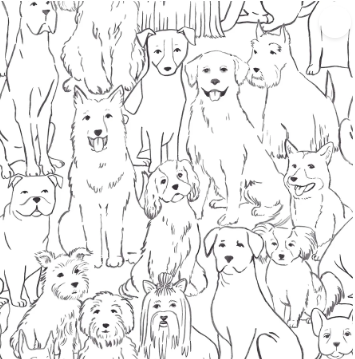
\includegraphics[width=0.8\textwidth]{mutts}

    \vspace{.3in}
    {\bfseries\Large
        August 2024\\
        \vskip2cm
        Rob McLaren, Young-jin Park, Sorab Panday\\
    }

    \vfill
    \vfill
\end{titlepage}

\pagestyle{empty} \tableofcontents

\chapter{Introduction}\label{chapter:Introduction} This document describes a new \mfu\footnote{\url{https://www.gsienv.com/software/modflow-usg/modflow-usg/}}  development environment which has these features:
\begin{itemize}
    \item We refer to it as Modflow User Tools, or \mut\ for short.
    \item \mut\ is designed to work with a modified version of \mfu,  where a new surface water flow package, called \swf, has been added. Like the Connected Linear Network (\cln) package, the \swf\ package represents a new domain type that is fully-coupled to the 3D groundwater flow (\gwf) domain. There can also be cell-to-cell flows between the \swf\ and \cln\ domains.  The \swf\ domain uses the diffusion-wave approach so simulate 2D surface-water flow. We will refer to this new version of \mfu\ as \mfus\ in this manual.
    \item We currently develop and run it on a \windows\ 10-based computing platform, writing software using the \ifort\ compiler running inside the \vstudio\ interactive development environment, which includes software version control tools through \github.
    \item A text-based approach is used for the \mut\ interface, in which we first develop an input file of instructions that define our \mfus\ project,  then run \mut\ to read it and write a complete \mfus\ data set. \mut\ also writes output files for \tecplot, a third-party visualization software package, which provides a 3D graphical visualization tool to review the model numerical mesh and material properties in the data set. In future, \mut\ could be extended to support other third-party visualization packages, for example the open source program Paraview.
    \item \mut\ can post-process a \mfus\ simulation to provide a \tecplot\ visualization of temporal model results, including hydraulic heads, saturations, water depths and flow budget data.  \textit{If applied to output files which were produced by an earlier version of Modflow, results may be mixed.  It is not our intent here to support all existing Modflow packages, many of which have been superceded.}
\end{itemize}

This document is subivided into these sections:
\begin{description}
    \item[Chapter~\ref{chapter:Installation}]\textbf{Installation and Setup:} How to install \mut, \mfus\ and \tecplot\ and define \windows\ environment variables.
     \item[Chapter~\ref{chapter:ModelBuild}]\textbf{\mut\ Execution and Pre-processing} How to build a \mut\ input file, produce a \mfus\ compatible data set and \tecplot\ compatible output files with \mut, then review the results of the model build with \tecplot.
    \item[Chapter~\ref{chapter:ModelExecution}]\textbf{\mfus\ Execution and Post-Processing} How to run \mfus, convert the output to \tecplot-compatible files with \mut, then visualize them with \tecplot.
    \item[Chapter~\ref{chapter:ModelVerification}]\textbf{Model Verification} Examples used to verify the accuracy of \mfus\ models built using \mut.
    \item[Chapter~\ref{chapter:IllustrativeExample}]\textbf{Illustrative Example} An example which illustrates the use of \mut\ and \mfus\ to simulate variably-saturated, fully-coupled   \gwf\-\swf\ flow in a large-scale watershed.
    \item[Appendix~\ref{Appendix:ExcelUseage}]\textbf{\excel\ Database Files} Details about using the provided \excel\ database files, which are currently used to store \mfus\ model material property and solver parameter data sets.
    \item[Appendix~\ref{Appendix:TecplotUseage}]\textbf{\tecplot\ Useage} Details about using \tecplot\ to visualize output files generated by \mut\ during model build and execution.
        \end{description} 

\chapter{Software Installation and Useage}\index{Installation}
\begin{enumerate}
    \item Obtain the MUT source files from:
        \begin{verbatim}
            https://github.com/Grdbldr/MUT_Source.git
            https://github.com/Grdbldr/MUT_Examples.git
        \end{verbatim}

    \item Define a windows environment variable USERBIN e\.g\.:
        \begin{verbatim}
            set USERBIN=c:\program_files\bin
        \end{verbatim}
        This can be done through Windows settings or at the command prompt.

    \item Build the source in Microsoft Visual Studio.  We provide a Visual Studio 2019 solution file for this purpose. Currently, Microsoft is providing a free community version of Visual Studio 2022 but we haven't yet tested this version.  Please let us know how this works if you try it.

\end{enumerate}   

\chapter{Model Build}\label{chapter:ModelBuild}
The first step in any model build is to develop a conceptual model, which defines the extent, inflows and outflows, material distributions and physical properties of a hydrogeologic flow system, real or imaginary. The intent of \mut\ is to then facilitate the production of a set of \mfus\ input files by minimizing the amount of time we spend building and testing it.  This chapter describes our current model build workflow, which can provide a sound basis for developing your own personal workflow.

The steps in our model build workflow are:
\begin{enumerate}
    \item Create a new working folder or copy an existing \mut\ project folder. \label{step:copy}
    \item Modify the \mut\ input file (and other input files if necessary) to reflect the new Modflow project.\label{step:modify}
    \item Run \mut\ to build the new Modflow project, which also produces \tecplot\ output files for the various Modflow domains (i.e. \gwf, \swf\ and/or \cln ) created during the build process. \label{step:mut1}
    \item Run \tecplot\ and examine the build output files.   \label{step:Tecplot1}
    \item Repeat steps~\ref{step:modify}-\ref{step:Tecplot1} until the new project is defined to your satisfaction.
\end{enumerate}

A \mut\ input file is a plain ascii text file that you can edit with your preferred editor (e.g. Windows Notepad\footnote{Our personal favourite editor is WinEdt (\url{https://www.winedt.com/snap.html}), which also provides a nice \LaTeX\ document development environment when coupled with the \TeX\ software package MiKTeX.  This manual was produced using these word processing tools.}).
The \mut\ input file name can have a prefix of your choice, followed by the extension \texttt{.mut}. Examples of valid \mut\ input file names are \texttt{\_build.mut} or \texttt{good.mut}. Most often, the easiest approach is to copy an existing input file and modify it as required.  This helps reduce set-up time and avoid potential errors that are introduced when creating input files from scratch.

To illustrate our model build workflow, we will refer to the various conceptual models developed for our existing suite of examples described in  Chapter~\ref{chapter:ModelVerification}.  As you read along, we urge you to carry out the steps we describe as we move through the workflow.  We recommend copying the contents of an existing model to a new location (e.g.\ copy the folder \texttt{1\_VSF\_Column} to \texttt{C:$\backslash$SandBox}).
\pagebreak 
If you did so, your working directory would look something like this:

    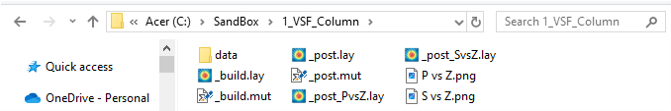
\includegraphics[width=\textwidth]{3_1_vsf_column_folderinit}

In the \texttt{1\_VSF\_Column} example, there is a \mut\ input file for the model build called \texttt{\_build.mut} and a \tecplot\ layout file called \texttt{\_build.lay} used to visualize the model build results.  The rest of the files are related to post-processing \mfus\ model results and will be discussed later in chapter~\ref{chapter:ModelExecution}.
 
 In our preferred workflow we would first start a command prompt in the folder which contains the \mut\ input file by:
\begin{enumerate}
   \item  Navigating to the folder in File Explorer (e.g.\ \texttt{C:$\backslash$SandBox$\backslash$1\_VSF\_Column}).
   \item  Highlighting the path in File Explorer:

        
\includegraphics[width=0.3\textwidth]{3_3_HighlightPath}

    \item  Replacing the existing path with the string {\sf cmd}:

        
\includegraphics[width=0.5\textwidth]{3_4_cmd}

    \item Pressing Enter/Return.
\end{enumerate}
A command prompt window rooted at the input folder should appear:

        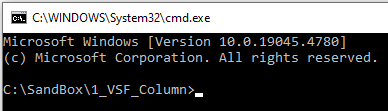
\includegraphics[width=0.4\textwidth]{3_5_cmdPrompt}



When you run \mut\, it will try to obtain a prefix in the following order:
\begin{enumerate}
    \item \textbf{From a command line argument:} \label{commarg} At the command prompt, \mut\ checks for the presence of a command line argument.  For example, typing this:
\begin{verbatim}
    mut Good
\end{verbatim}
        would cause \mut\ to process the input file \texttt{Good.mut}.
    \item \textbf{From a prefix file:} If there is no command line argument, \mut\ checks for the presence of the file \texttt{\_mut.pfx} in the folder.  If present, \mut\ will read the prefix from it. For example, if the mut file was called \texttt{Good.mut} then the file \texttt{mut.pfx} would contain the single line:
\begin{verbatim}
    good
\end{verbatim}
    \item \textbf{From the default input file:} If there is no command line argument or prefix file in the folder, \mut\ checks for the presence of the file \texttt{a.mut}.  If present in the folder, \mut\ will process it.
    \item \textbf{From the keyboard:} If none of these methods are successful, \mut\ will prompt for a prefix as shown here:

        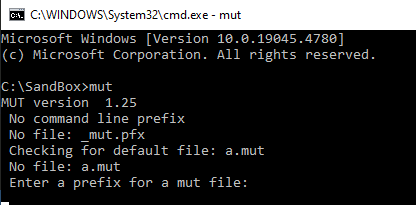
\includegraphics[width=0.6\textwidth]{3_2_mut_no_prefix}

        The user would type the prefix e.g.: \texttt{good} and press Enter.

\end{enumerate}

To build the \texttt{1\_VSF\_Column} example, we would  run \mut\ using the input file \texttt{\_build.mut} by typing:
\begin{verbatim}
    mut _build
\end{verbatim}
which uses the first method to supply the prefix.


If you open the file \texttt{\_build.mut} in a text editor you will see the first couple of lines are comments (which begin with an exclamation point character: '{\tt !}') describing the problem:
\squish
\begin{verbatim}
    ! Examples\1_VSF_Column:
    !   A modflow project of a 1D column generated from a simple 2d rectangular mesh
\end{verbatim}
 \mut\ first creates a clean copy of the input file called \texttt{\_buildo.input} by removing all comment lines.

 As \mut\ processes the input file, output is written to both the screen and to the file \texttt{\_buildo.eco}.  If you open \texttt{\_buildo.eco}, you will see the first thing written is the \mut\ header, which contains the version number and build date.

 These are followed by the stripped comments, which  can provide a synopsis of the input file contents. The rest of the cleaned input file contains \mut\ instructions, which may require data in the form of numbers (e.g.\ parameter values) or alphanumeric strings (e.g.\ file names).


The first instruction in the cleaned input file begins the model build:

\ins{build modflow usg}
    {This  is a {\em subtask} that defines the characteristics of the \mfus\ model including:
     \begin{itemize}
        \item Units of length and time.
        \item Numerical model meshes.
        \item Material properties.
        \item Boundary conditions.
        \item Time-stepping, stress period and output control parameters.
        \item Solver parameters.
    \end{itemize}

    An end instruction is required to stop the subtask e.g.:

    {\Large \sf end build modflow usg}
    }

After \mut\ finishes, the working folder should look something like this:

        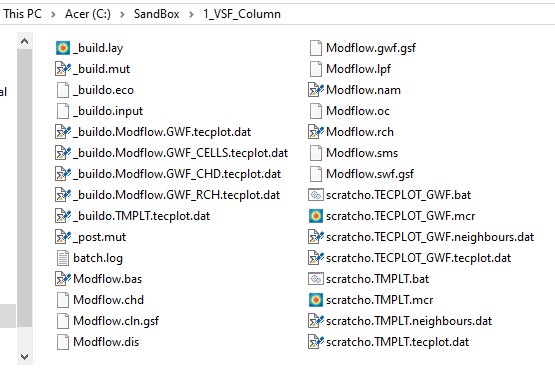
\includegraphics[width=0.8\textwidth]{3_6_buildFiles}

Several new output files have been created, of which it may be noted:
\begin{itemize}
    \item Build output files, which have the prefix \texttt{\_buildo}, appear near the start of the list if sorted by name. \mut\ deletes previously generated build output files and writes a fresh set each time it is run.  This can prevent confusion that might arise if out-of-date output files were present.\footnote{For example, if we define a recharge boundary condition, \mut\ will create the file \texttt{\textit{prefix}o.Modflow.SWF\_RCH.Tecplot.dat} which shows the locations and recharge values assigned to Modflow cells.  If we then removed the recharge condition from the input file, but did not delete this output file, we may assume the recharge condition still applies.}
    \item \tecplot\ output files are indicated by the suffix \texttt{.tecplot.dat}.
    \item Modflow model input files are written using the default prefix \texttt{Modflow}, (e.g.\ \texttt{Modflow.nam, Modflow.bas} etc.)  The prefix can be customized if desired but there are advantages to keeping this 'generic' one, such as portability of post-processing scripts or \tecplot\ layout files that follow this generic naming convention.
    \item Several scratch files (with prefix \texttt{scratcho}) are written. These are used for debugging during code development and can be ignored in most cases.
    \item If the run is successful the last line written will be \texttt{Normal exit}, otherwise an error message will be given.
\end{itemize}


    \section{Suggested Workflow}\label{Appendix:SuggestedWorkflow}A well-designed workflow should minimize the introduction of human error into the modelling process and facilitate later review by senior modellers.   Below we describe one possible approach that can be used as a starting point for implementing your own personal workflow.  We will use the verification example \verb+6_Abdul_Prism_Cell+ to demonstrate our suggested workflow. The steps in the workflow are:
\begin{enumerate}
    \item Copy an existing \mut\ project folder to a new working folder. \label{step:copy}
    \item Modify the \verb+_build.mut+ file (and other input files if necessary) to reflect the new Modflow project.\label{step:modify}
    \item Run \mut\ to build the new Modflow project, which produces \tecplot\ output files for the various Modflow domains (i.e. GWF, SWF and/or CLN) created during the build process. \label{step:mut1}
    \item Run \tecplot\ and examine the build output files.   Repeat steps~\ref{step:modify}-\ref{step:mut1} until the new project is defined correctly.\label{step:Tecplot1}
    \item Run Modflow to create the new project output files (e.g.\ time-varying hydraulic head, drawdown etc).\label{step:modflow}
    \item Run \verb+_post.mut+ to post-process the Modflow project, which produces \tecplot\ output files for the various Modflow domains (i.e.\ GWF, SWF and/or CLN) created during the Modflow simulation.\label{step:mut2}
    \item Run \tecplot\ and examine the Modflow output files.   \label{step:Tecplot2}
\end{enumerate}


    \section{\mut\ Input File Structure}\label{tex:InputFile}
\mut\ recognizes files which have the extension \verb+.mut+ as input files and reads and interprets them to produce both \mfus\ output files and \tecplot\ input files. Input files are ordinary text files which contain comments, \mut\ instructions and data which can be numbers or alphanumeric strings.

Comments begin with an exclamtion point character \verb+!+ and are ignored by \mut.  \mut\ initially strips the input file of all comments and creates a clean copy called \textit{prefix}\verb+o.input+, which is then processed by \mut.  This means comments can be placed anywhere in the input file.



    \section{\tecplot\ Useage}\label{tecfile:TecplotUseage} 
    \section{Groundwater Flow(GWF) Domain}\label{texfile:GWF}
Currently, every \mfus\ model must contain a \gwf\ domain, which may be reduced to a single layer of very low hydraulic conductivity in cases where \gwf\ flow and interaction with other model domains is to be neglected.

\subsection{Generating a Layered \gwf\ Domain}
A \mfus\ 3D groundwater flow (\gwf) domain can be generated from the template using this instruction:

\ins{generate layered gwf domain}
    {This subtask has instructions that are used to define:
     \begin{itemize}
        \item Element zone numbering scheme
        \item Top elevation (i.e. $z$-coordinate)
        \item Mesh layers and vertical discretization
    \end{itemize}

    Subtask instructions will be read and processed until an \textsf{end} instruction is encountered.  We suggest appending the subtask name to the \textsf{end} instruction:

    {\Large \sf end generate layered gwf domain}
    }

The construction of the 3D \gwf\ finite-element mesh proceeds from top to bottom.  First, we define the top elevation, then add layers one at a time until we reach the base of the domain. By default, element zone numbers will be assigned by layer number.  If the template mesh is divided into horizontal patches with unique zone numbers, these can be assigned instead to the 3D GWF mesh \footnote{The verification example \texttt{MUT\_Examples$\backslash$6\_Abdul\_Prism\_Cell} uses this option to define \swf\ domain zones.} using this instruction:

\ins{Zone by template}
    {Causes \mut\ to assign the template mesh element zone number to the corresponding 3D \gwf\ element.

    {\em This instruction should appear in the input file at the beginning of the \textsf{generate layered gwf domain} subtask before new layers are added.}
    }

\subsubsection{Defining the Top Elevation} \label{section:topelev}
To assign an elevation to the top layer of template nodes use this instruction:

\ins{top elevation}
    {This subtask defines the elevation (i.e. $z$-coordinate) of the top layer of nodes in the \gwf\ finite-element template mesh in one of these ways:
     \begin{itemize}
        \item By assigning a given elevation to all nodes
        \item By reading variable elevation data from a file
        \item By interpolating elevation data from a function $z(x)$ where the elevation $z$ varies by the nodes $x$ coordinate.
     \end{itemize}
     Once the elevation is defined, an \textsf{end} instruction is required to stop the subtask e.g.\:

    {\Large \sf end top elevation}
    }

 The top elevation can be defined by one of these instructions: \label{'Page:TopElev'}

 \ins{elevation constant}
    {\squish
    \begin{enumerate}
    \item \rnum{elev}\  The elevation \rnum{elev}\ will be assigned to all top layer nodes.
    \end{enumerate}
    \squish
    }

 \ins{elevation from gb file}
    {\squish
    \begin{enumerate}
    \item \str{file}\  The elevation data in the \gb\ nodal property file named \str{file}\ will be assigned to the top layer nodes.
    \end{enumerate}
    \squish
    }

The \gb\ nodal property file uses a legacy binary file format. You can develop your own ascii input files and read them using this instruction:

 \ins{elevation from list file}
    {\squish
    \begin{enumerate}
    \item \str{file}\  The elevation data in the ascii file named  \str{file}\ will be assigned to the top layer nodes.
    \end{enumerate}
    \squish
    }

Part of a sample list file \footnote{The verification example \texttt{MUT\_Examples$\backslash$6\_Abdul\_MODHMS} uses an ascii file input to define nodal elevations.} is shown here:
    \begin{verbatim}
    Kriged cell top elevation for layer 1
     4.414571762E+000
     4.415914536E+000
     ...
     4.415914536E+000
     \end{verbatim}
     \squish
Some key features of this example are:
\begin{itemize}
  \item The first line of the file is discarded, and in this case contains a string describing the data.
  \item You must supply a value for each node in the template finite-element mesh.
  \item The data is read in free format so there can be more than one value entered per line.
  \item Only the start and end of the file are shown here, with the string '\texttt{...}' replacing the middle portion.
\end{itemize}

To define the top elevation as a function of $x$ (usually used for cross-sectional models) use this instruction:

 \ins{elevation from xz pairs}
    {
    \squish
    \begin{enumerate}
    \item \rnum{x(1)}, \rnum{y(1)}  First $x, z$ coordinate pair.
    \item \textbf{...}
    \item \rnum{x(n)}, \rnum{y(n)}  nth $x, z$ coordinate pair.
    \end{enumerate}

     An elevation is calculated for each chosen cell, based on it's $x$-coordinate location, by interpolating an elevation from the given list of  $xz$-coordinate pairs.

     This subtask reads a list of $xz$-coordinate pairs until an \textsf{end} instruction is encountered e.g.\:

    {\Large \sf end elevation from xz pairs}
    }

Here is an example showing the use of this instruction \footnote{The verification example \texttt{MUT\_Examples$\backslash$1\_VSF\_Hillslope} uses the \textsf{elevation from xz pairs} pairs instruction to define the top elevation of the cross-sectional domain.}:
    \begin{verbatim}
    elevation from xz pairs
           0.0, 0.0
        1000.0, 100.0
    end elevation from xz pairs
     \end{verbatim}
     \squish
Some key features of this example are:
\begin{itemize}
  \item The two given $xz$ pairs define a line that slopes from $z=0$ at $x=0$ to $z=100.0$ at $x=1000$.  You may supply as many pairs as needed to define the top of your cross-section.
  \item $x$ coordinates must increase continuously from the top of the list to the bottom.
  \item the $x$-range of the supplied pairs should cover the entire $x$-range of the template mesh.
  \item For each node in the template mesh, the $x$ coordinate is used to interpolate an elevation (i.e. $z$ value) using the appropriate $xz$ pair.
\end{itemize}

\subsubsection{Adding Layers} \index{\gwf\ Domain ! layering}
    {\em NOTE: The term layers used here should not be confused with the \mf\ term of the same name. A \mf\ layer is one cell thick, while a \mut\ layer can be one or more elements thick.}

A \mfus\ model must contain at least 1 layer, and each layer is defined using this instruction:     {\index{Grid generation ! \gwf\ Domain ! New layer}

\ins{new layer}
    {This subtask adds a new layer to the \gwf\ domain by defining the layer:
     \begin{itemize}
       \item Base elevation
       \item Vertical discretization
     \end{itemize}

     It reads instructions until an \textsf{end} instruction is found e.g.\:

    {\Large \sf end new layer}
    }

The base elevation is defined using the elevation instructions  described on page~\pageref{'Page:TopElev'} that are given for the \textsf{top elevation} instruction.

By default, a new layer will be assigned the name '\texttt{Layer {\em n}}' where {\em n} is the current layer number.  If you want to assign your own layer name use this instruction:

\ins{Layer name}
    {
    \squish
    \begin{enumerate}
    \item \str{layer\_name} Layer name.
    \end{enumerate}
    \squish
    }

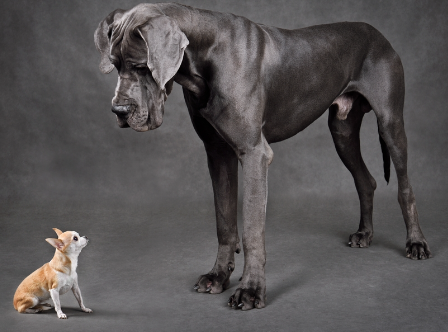
\includegraphics[width=.15\textwidth]{ModelDevelopment} \textit{These names are not currently used in Tecplot output but could/should? be used to create the customlables for zone naming.}



By default, \mut\ will stop and issue a warning message if the computed layer base elevation is greater than or equal to the current layer top elevation.  This instruction forces the base to be below the top by a set amount:

\ins{Minimum layer thickness}
    {\squish
    \begin{enumerate}
    \item \rnum{MinThick} Minumum thickness value[L].
    \end{enumerate}
    This instruction causes \mut\ to enforce a minimum thickness constraint for the current layer. At nodes where the computed layer base elevation is greater than or equal to the current top elevation, \rnum{MinThick} will
    be subtracted from the current top elevation to get the base elevation.
    }

By default, a new layer will not be subdivided vertically unless one the following two instructions is issued.
The first creates a uniform subdivision:

\ins{Uniform sublayering}
    {\squish
    \begin{enumerate}
    \item \inum{nsublayer} Number of sublayers.
    \end{enumerate}
    This instruction divides the layer vertically into \inum{nsublayer}
    elements, which will each have the same element height, equal to the top elevation
    minus the current base elevation divided by \inum{nsublayer}.
    }

This instruction creates a non-uniform subdivision:

\ins{Proportional sublayering}
    {\squish
    \begin{enumerate}
        \item \inum{nsublayer}  Number of proportional sublayers.
        \item \rnum{sub\_thick(i),i=1,\inum{nsublayer}} Proportional thicknesses in order from top to bottom.
    \end{enumerate}
    This instruction can be used if you want to refine the \gwf\ domain mesh vertically,
    for example, in the active zone with the \swf\ domain the ground surface in the .

    It is important to understand that the variable \rnum{sub\_thick} is not
    a true thickness, but is instead a relative thickness, which is used along
    with the layer thickness to determine the element heights in the current
    column.

}

    For example, these instructions:
    \texttt{
            \begin{tabbing}
            AAA\=AAA\=AAA   \kill
                \>Proportional sublayering   \\
                \>   \> 3                     \\
                \>   \> 0.1           \\
                \>   \>1.0            \\
                \>   \>  10.0       \\
                \> end       \\
            \end{tabbing}
    }
    \squish
would subdivide the current layer vertically into three elements, between
    the current base and top elevation, with element height proportions of .1,
    1 and 10 from top to bottom.

This instruction is most often used to define a layer of uniform thickness relative to an uneven top elevation:

\ins{Offset base}
    {\squish
    \begin{enumerate}
    \item \rnum{value} Thickness value (L) by which to offset the layer base elevation.
    \end{enumerate}
    This instruction causes the elevation of the base of the layer to be offset vertically by the given value.  This
    can be used to create a surface a given distance below another surface.
}

    For example, these instructions:
\begin{verbatim}
        top elevation
            elevation from list file
            elev.list
        end top elevation

        new layer
            uniform sublayering
            3

            elevation from list file
            elev.list

            offset base
            -1.0

        end new layer

    end generate layered gwf domain
\end{verbatim}
 create a layer with a top elevation 1 metre below the elevation defined in the raster file \texttt{elev.list}:


\includegraphics[width=.15\textwidth]{UnderConstruction} \textit{Need to check sign on \textsf{offset base} input}

\subsubsection{Cell Connection Properties}  \index{\gwf\ Domain ! cell connection properties}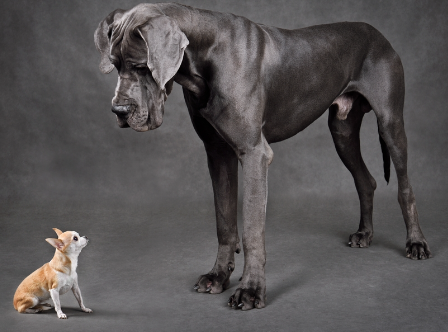
\includegraphics[width=.15\textwidth]{ModelDevelopment} \textit{
\gwf\ cell to \gwf\ cell connection properties are automatically defined by \mut\ based on control-volume approach and element type. The code needs to be checked, verified and documented more completely.}



\subsubsection{Assigning Material Properties}  \index{\gwf\ Domain ! material properties}

\gwf\ domain material properties may vary on a cell-by-cell  basis.  \mut\ offers some simple instructions for selecting cells and assigning material property values to them.  As you might imagine, this instruction:

\ins{choose all cells}
    {Select all cells in the active model domain.
     }

selects all cells in the {\em active} model domain.

This is an example of what we refer to as a {\em generic} instruction, which means it can be applied to any of the currently available model domains: \gwf, \swf\ or \cln.

If our intention is to choose all cells in the \gwf\ domain, we first need to activate it using this instruction:

\ins{active domain}
    {
        \squish
        \begin{enumerate}
        \item \str{Domain}  The name of the domain to be activated: \gwf, \swf\ or \cln\
        \end{enumerate}
        This instruction activates the given domain named in  \str{Domain} so that it will be used with generic instructions such as \textsf{choose all cells}.
    }

So to activate the \gwf\ domain, we would insert these instructions in the input file:
\begin{verbatim}
    active domain
    gwf
\end{verbatim}

These instructions can be used to choose cells in various ways\label{page:cellSelect}:

\ins{choose cell at xyz}
    {
        \squish
        \begin{enumerate}
        \item \rnum{x1}, \rnum{y1}, \rnum{z1}  An $xyz$ coordinate triplet.
        \end{enumerate}
        The cell closest to the given $xyz$ coordinate triplet will be chosen.
    }

\ins{choose cells by layer}
    {
        \squish
        \begin{enumerate}
        \item \inum{layer}  The number of the layer to be chosen.
        \end{enumerate}
        The cells in Modflow layer number \inum{Layer} will be chosen.  Remember that Modflow layers are one cell high and are numbered from the top to the bottom of the model domain.\footnote{ See the verification example \texttt{MUT\_Examples$\backslash$1\_VSF\_Column} which uses the previous two instructions to define a constant head at  the base  and a recharge boundary condition at the top of the 1D column.}
    }

\ins{choose cells from file}
    {
        \squish
        \begin{enumerate}
        \item \str{file}  The file \str{file} containing a list of cell numbers.
        \end{enumerate}
        The cells listed in the file \str{file} will be chosen.  \footnote{ See the verification example \texttt{MUT\_Examples$\backslash$1\_Abdul\_MODHMS} which uses this instruction to assign some cells as inactive.}
    }

\pagebreak
\ins{choose cells from gb elements}
    {
        \squish
        \begin{enumerate}
        \item \str{file}  The \gb\ chosen element file \str{file} containing information concerning the status, chosen or not chosen, of each element in the \gb\ model domain.
        \end{enumerate}
          If an element is flagged as chosen in the \gb\ model domain then the corresponding cell will be chosen in the \mfus\ model domain.  \footnote{ See the verification example \texttt{MUT\_Examples$\backslash$1\_Abdul\_Prism\_Cell} which uses this instruction to assign some cells as inactive.}
    }

\ins{choose cells from gb nodes}
    {
        \squish
        \begin{enumerate}
        \item \str{file}  The \gb\ chosen node \str{file} containing information concerning the status, chosen or not chosen, of each node in the \gb\ model domain.
        \end{enumerate}
          If a node is flagged as chosen in the \gb\ model domain then the corresponding cell will be chosen in the \mfus\ model domain.  \footnote{ See the verification example \texttt{MUT\_Examples$\backslash$1\_Abdul\_Prism\_Cell\_nc} which uses this instruction to assign some cells as inactive.}
    }

The previous two instructions are used to choose cells for the mesh-centered and node-centered approaches respectively.

Cell selection instructions are cumulative.  For example, you can modify the current selection by repeating instructions like  \textsf{choose cell at xyz} or \textsf{choose cells by layer} with different inputs and then assign properties to the current selection.  This instruction clears the selection before beginning new cell selection(s):

\ins{clear chosen cells}
    {Clears the current cell selection.
     }

It is good practice to clear the selection before starting a new selection. \mut\ echoes the results of the selection instructions to the screen and \texttt{.eco} file as shown in this example:
\begin{verbatim}
    clear chosen cells
    	GWF Cells chosen:          0

    choose all cells
    	GWF Cells chosen:      39765
\end{verbatim}
If a cell selection instruction has unexpected results these are good places to check.

\pagebreak
These instructions can be used to assign material properties to the current cell selection:

\ins{gwf kh}
    {
        \squish
        \begin{enumerate}
        \item \rnum{val}  Horizontal hydraulic conductivity [$L$   $T^{-1}$].
        \end{enumerate}
          A horizontal hydraulic conductivity of \rnum{val} is assigned to the chosen cells.
    }


\ins{gwf kv}
    {
        \squish
        \begin{enumerate}
        \item \rnum{val}  Vertical hydraulic conductivity [$L$   $T^{-1}$].
        \end{enumerate}
          A vertical hydraulic conductivity of \rnum{val} is assigned to the chosen cells.
    }

\ins{gwf ss}
    {
        \squish
        \begin{enumerate}
        \item \rnum{val}  Specific storage [$L^{-1}$].
        \end{enumerate}
          A specific storage of \rnum{val} is assigned to the chosen cells.
    }

\ins{gwf sy}
    {
        \squish
        \begin{enumerate}
        \item \rnum{val}  Specific yield (-).
        \end{enumerate}
          A specific yield of  \rnum{val} is assigned to the chosen cells.
    }

\ins{gwf alpha}
    {
        \squish
        \begin{enumerate}
        \item \rnum{val}  Van Genuchten/Brooks-Corey Alpha [$L^{-1}$].
        \end{enumerate}
          A Van Genuchten/Brooks-Corey Alpha of \rnum{val} is assigned to the chosen cells.
    }

\ins{gwf beta}
    {
        \squish
        \begin{enumerate}
        \item \rnum{val}  Specific yield (-).
        \end{enumerate}
          A specific yield of \rnum{val} is assigned to the chosen cells.
    }

\ins{gwf sr}
    {
        \squish
        \begin{enumerate}
        \item \rnum{val}  Residual saturation [-].
        \end{enumerate}
          A residual saturation of \rnum{val} is assigned to the chosen cells.
    }

\ins{gwf brooks}
    {
        \squish
        \begin{enumerate}
        \item \rnum{val}  Brooks-Corey exponent.
        \end{enumerate}
          A Brooks-Corey exponent of \rnum{val} is assigned to the chosen cells.
    }

Defining each different material property as described above can be tedious.  A lookup table of \gwf\ material properties  is provided in the file \texttt{qryGWFMaterials.txt}, located in the \bin\ directory as outlined on page~\pageref{page:userbin}.

In order for \mut\ to access the lookup table, you first need to provide a link to this file using the instruction:

\ins{gwf materials database}
    {
        \squish
        \begin{enumerate}
        \item \str{file}  \gwf\ material properties lookup table file name.
        \end{enumerate}
          \mut\ uses the file \str{file} to look up \gwf\ material properties.
    }

You can now assign a full set of \gwf\ material properties to the current cell selection, as described on page~\pageref{page:cellSelect}, using this instruction:

\ins{chosen cells use gwf material number}
    {
        \squish
        \begin{enumerate}
        \item \inum{val}  \gwf\ material ID number.
        \end{enumerate}
          A unique set of \gwf\ material properties is retrieved from a lookup table, using the given  material ID number \inum{val}, and assigned to the chosen cells.
    }

You can find detailed information about how to use \dbase\ to modify or define your own lookup tables in Tutorial~\ref{tecfile:DbaseUseage}.

\pagebreak
During the model build, each \gwf\ cell is assigned a zone number from either the layer number or 2D template zone number. Just like individual cells, zones can be selected using these instructions\label{page:zoneSelect}:

\ins{choose all zones}
    {Select all zones in the active model domain.
     }

\ins{choose zone number}
    {
        \squish
        \begin{enumerate}
        \item \inum{value}  The number of the zone to be chosen.
        \end{enumerate}
        \squish
    }

\ins{clear chosen zones}
    {Clears the current zone selection.
     }

The zone selection can be converted into a cell selection using this instruction:

\ins{choose cells by chosen zones}
    {If a zone is currently chosen, any cell which has that zone number will be chosen.
     }
This cell selection can now be used to assign material properties.

Below is an example \footnote{See verification example \texttt{MUT\_Examples$\backslash$6\_Abdul\_Prism\_Cell}} of a case in which the element zone numbers have been assigned by layer number for a 3-layer case:

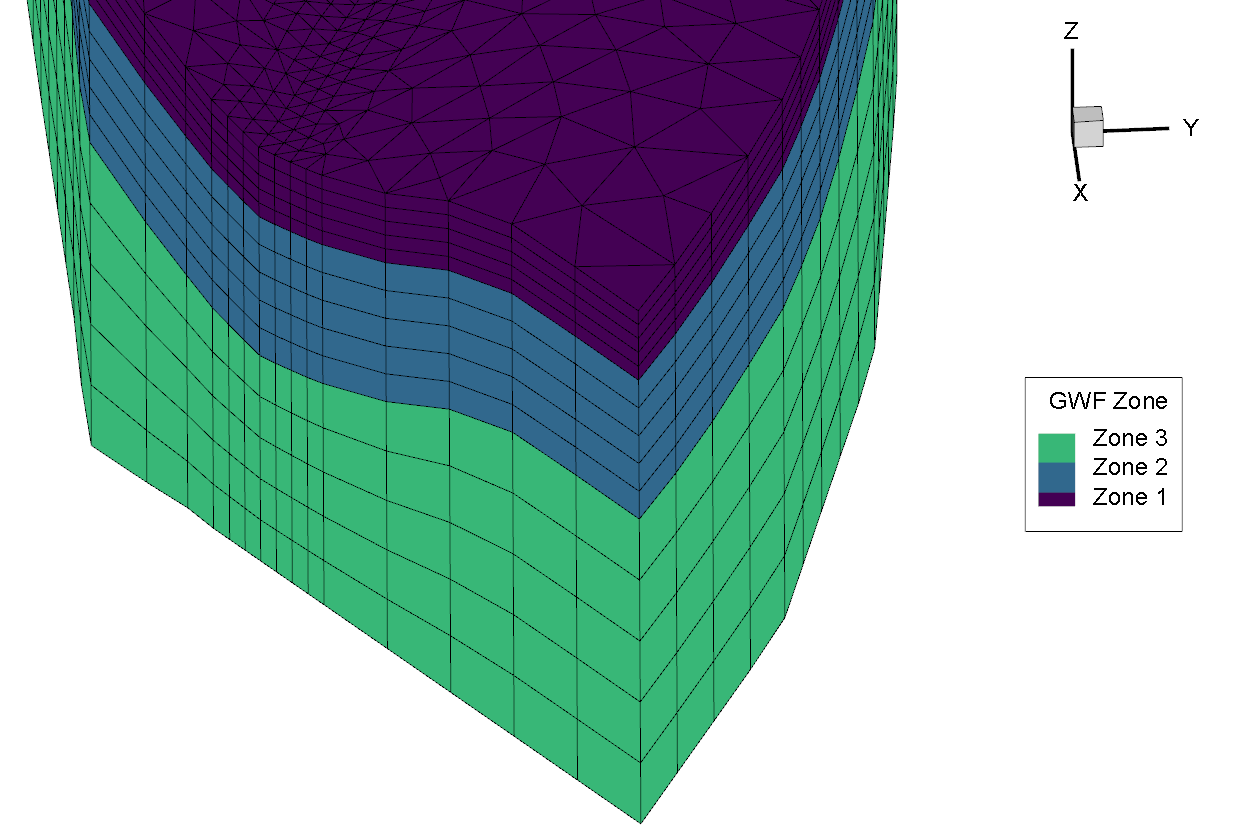
\includegraphics[width=.86\textwidth]{3_10_GWFZones}

\pagebreak
Some key features to note are:
\begin{itemize}
    \item There are 3 zones, corresponding to the layers 1 to 3.
    \item 'Zone 1', coloured dark blue, corresponds to layer 1.  Recall that the \mfus\ mesh is generated from the top down, so layer 1 is at the top of the model domain.
    \item Each layer is composed of multiple \mf\ layers, which are each one cell thick.
\end{itemize}

The following example uses the materials database and zone selection to assign material properties for the 3-layer case:

\begin{verbatim}
    gwf materials database
    	Materials file C:\MUT\MUT_Examples-main\_MUT_USERBIN\qryGWFMaterials.txt

    active domain
    	gwf

    clear chosen zones
    	GWF Zones chosen:          0

    choose zone number
    	Adding zone number:        1
    	GWF zone numbers currently chosen:
    	    1

    choose zone number
    	Adding zone number:        2
    	GWF zone numbers currently chosen:
    	    1
    	    2

    choose zone number
    	Adding zone number:        3
    	GWF zone numbers currently chosen:
    	    1
    	    2
    	    3

    clear chosen cells
    	GWF Cells chosen:          0

    choose cells by chosen zones
    	GWF Cells chosen:      39765

    chosen cells use gwf material number
    	Assigning all chosen GWF cells properties of material               4, Borden sand
    	Kh_Kx:                 1.00000E-05
    	Kv_Kz:                 1.00000E-05
    	Specific Storage:      1.20000E-07
    	Specific Yield:        0.34000
    	Alpha:                  1.9000
    	Beta:                   6.0000
    	Sr:                    0.18000
    	Unsaturated Function Type:   Van Genuchten
\end{verbatim}

Some key features to note are:
\begin{itemize}
    \item As we choose zone numbers, the list of currently chosen zones grows accordingly.
    \item The final number of \gwf\ cells chosen is equal to the total number of cells in the domain, since we had selected all 3 layers prior to converting the  zone selection to a cell selection.
    \item After assignment, the \gwf\ material number, name and assigned property values are echoed to screen and \texttt{.eco} file.
\end{itemize}

\subsubsection{Initial Conditions}  \index{\gwf\ Domain ! initial condition ! initial (starting) head}
An initial (or starting) head should be assigned to each cell in the \gwf\ domain.  This could be an initial guess at the beginning of a transient stress period or a set of hydraulic heads from a previous run.

To assign a uniform hydraulic head to the \gwf\ model domain, you must first make a cell selection as described on page~\pageref{page:cellSelect}, then use this instruction:

\ins{gwf initial head}
    {
        \squish
        \begin{enumerate}
        \item \rnum{value}  Initial (or starting) hydraulic head [L].
        \end{enumerate}
          An initial hydraulic head  of \rnum{value} is assigned to the chosen cells.
    }

To assign a linearly varying head that is a function of $z$ (i.e.\ depth or elevation), use this instruction:
\ins{gwf initial head function of z}
    {
    \squish
    \begin{enumerate}
    \item \rnum{z(1)}, \rnum{head(1)}  First $z, head$ pair.
    \item \rnum{z(2)}, \rnum{head(2)}  Second $z, head$ pair.
    \item \textbf{...}
    \item \rnum{z(n)}, \rnum{head(n)}  nth $z, head$  pair.
    \end{enumerate}

     An initial head is calculated for each chosen cell, based on it's $z$-coordinate location, by interpolating a head from the given list of  $z, head$ pairs.

     This subtask reads a list of $z, head$ pairs until an \textsf{end} instruction is encountered e.g.\:

    {\Large \sf end gwf initial head function of z}
    }

This is commonly used to generate an initial head for a simple column model \footnote{The verification example \texttt{MUT\_Examples$\backslash$1\_VSF\_Column} uses the \texttt{gwf initial head function of z} instruction to define the initial head of the model domain} as shown here: :
\begin{verbatim}
    gwf initial head function of z
    !  z    head
      0.0  -100.0
    100.0     0.0
\end{verbatim}
Some key features of this example are:
\begin{itemize}
  \item The two given $z,head$ pairs define an initial head  that varies from $head=-100.0$ at $z=0$ to $head=0.0$ at $z=100.0$.  You may supply as many pairs as needed to define the initial head.
  \item $z$-coordinates must increase continuously from the top of the list to the bottom.
  \item the $z$-range of the supplied pairs should cover the entire $z$-range of the model domain.
  \item For each node in the model domain  mesh, the $z$ coordinate is used to interpolate an initial head (i.e. $head$ value) using the appropriate $z, head$ pair.
\end{itemize}

\subsubsection{Boundary Conditions}  \index{\gwf\ Domain ! boundary conditions}
A constant head boundary condition fixes the head at a \gwf\ cell at a given value, allowing water to flow into or out of the \gwf\ model domain depending on surrounding conditions.    To assign a uniform constant head to the \gwf\ model domain use this instruction:

\ins{gwf constant head}
    {
        \squish
        \begin{enumerate}
        \item \rnum{value}  Constant hydraulic head [L].
        \end{enumerate}
          An constant hydraulic head  of \rnum{value} is assigned to the chosen cells.
    }

A drain boundary condition allows water to flow out of the \gwf\ model domain if the hydraulic head of the cell is higher than the drain elevation.   To add a drain to the \gwf\ model domain use this instruction:

\ins{gwf drain}
    {
        \squish
        \begin{enumerate}
        \item \rnum{value}  Drain conductance [L/T].
        \end{enumerate}
          A drain conductance of \rnum{value} is assigned to the chosen cells.  The top elevation of the cell is assigned automatically as the drain elevation
    }

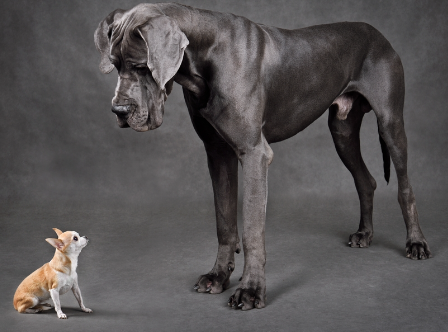
\includegraphics[width=.15\textwidth]{ModelDevelopment} \textit{Should we add an instruction where the drain elevation is specified?  }

A recharge boundary condition forces  water to flow in to the \gwf\ model domain at a specified rate.   To add a recharge  to the \gwf\ model domain use this instruction:

\ins{gwf recharge}
    {
        \squish
        \begin{enumerate}
            \item \rnum{value}  Recharge rate [L/T].
            \item \inum{option}  Recharge option.
        \end{enumerate}
        A recharge rate of \rnum{value} is assigned to the chosen cells.

        The recharge option \inum{option}is used to define where the recharge  is to be applied and can have one of the following values:
        \begin{enumerate}
            \item To top layer
            \item To one specified node in each vertical column
            \item To highest active node in each vertical column
            \item To the swf domain on top of each vertical column
        \end{enumerate}
        \squish
    }

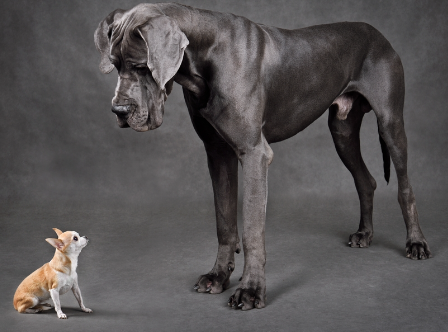
\includegraphics[width=.15\textwidth]{ModelDevelopment} \textit{Sould we have an example of pumping with an assigned nodal flux?  Should it be from a CLN?  Is there a boundary condition that assures the head will not be drawn down below the pumping node elevation?}






        \subsection{Constant Head(CHD)}    \index{Constant head CHD}
    \begin{verbatim}
    Pre-requisites:
    Activate one of GWF, SWF or CLN domains
    Choose cells

    Instructions:
    gwf constant head

    Inputs:
    Head    L
    \end{verbatim}

    All chosen cells will be assigned a constant head equal to the specified total head value.  
        \subsection{Drains(DRN)}\input{Drains}
        \subsection{Recharge(RCH)}
        \subsection{Pumping}
    \section{Connected Linear Networks(CLN) Domain}
    \section{Surface Water Flow(SWF) Domain}
        \subsection{Critical Depth}
        \subsection{Zero-Gradient Depth}

\chapter{Model Execution and Post-Processing}\label{chapter:ModelExecution}
The steps in our model excution  workflow are:
\begin{enumerate}
    \item Run \mfus to create the new project output files (e.g.\ time-varying hydraulic head, drawdown etc).\label{step:modflow}
    \item Run \mut\ to post-process the Modflow project, which produces \tecplot\ output files for the various Modflow domains (i.e.\ \gwf, \swf\ and/or \cln ) created during the Modflow simulation.\label{step:mut2}
    \item Run \tecplot\ and examine the Modflow output files.   \label{step:Tecplot2}
\end{enumerate}

To run \mfus\ on the \texttt{1\_VSF\_Column} example, and assuming we have a command prompt open at the appropriate directory, we can type:
\begin{verbatim}
    usgs_1 modflow
\end{verbatim}
which obtains the prefix for the \mfus\ input files, in this case the default prefix {\sf modflow}.

 As \mfus\ processes the input file, output is written to the screen:

        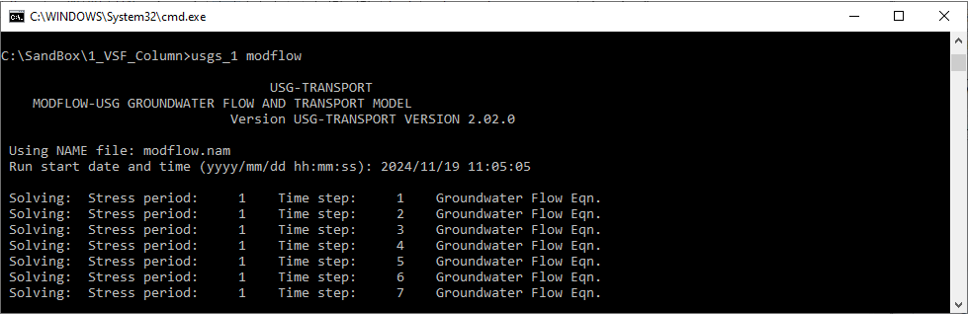
\includegraphics[width=\textwidth]{4_1_RunScreen}

 If execution is successful you will see the {\sf Normal termination of simulation} message:

        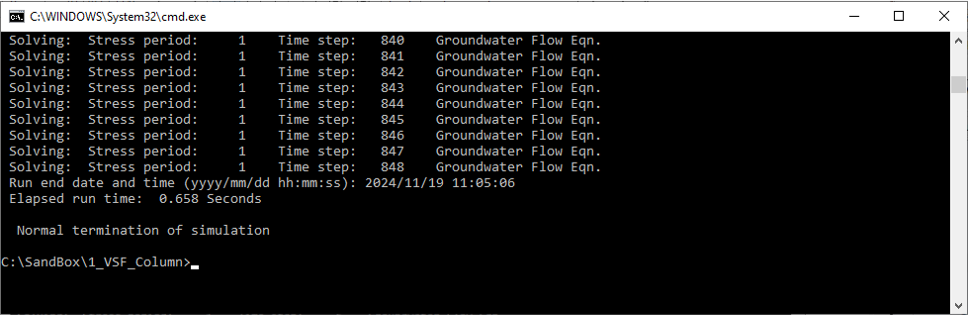
\includegraphics[width=\textwidth]{4_1_RunScreenExit}

 Every \mfus\ simulation generates a run-time
listing file, in this case called {\tt modflow.lst}, that consists of the input data for the simulation;
the solver and nonlinear outputs at user-requested detail; head
and drawdown solutions, if requested; mass-balance information; and time-step information for the simulation.  It also produces binary files of head, drawdown, saturation and cell-by-cell flows for each model domain.

To post-process the output produced by \mfus\ for the \texttt{1\_VSF\_Column} example, we would  run \mut\ using the input file \texttt{\_post.mut} by typing:
\begin{verbatim}
    mut _post
\end{verbatim}

If you open the file \texttt{\_post.mut} in a text editor you will see the first  line is a comment followed by one instruction and input:
\squish
\begin{verbatim}
    ! This example reads a modflow project and postprocesses it
    postprocess existing modflow model
        modflow
\end{verbatim}
As in the model build, \mut\ first creates a clean copy of the input file called \texttt{\_posto.input} by removing all comment lines.
 As it processes the input file, output is written to both the screen and to the file \texttt{\_posto.eco}.

The instruction to post-process the \mfus\ model after execution is:

\ins{postprocess existing modflow model}
    {
        \squish
        \begin{enumerate}
        \item \str{Prefix}  The \mfus\ model prefix.
        \end{enumerate}
        Given \str{Prefix}, this instruction:
         \begin{itemize}
            \item  Reads head, drawdown and cell-by-cell flow binary output files for each output time and writes the results to the file {\tt \_posto.modflow.GWF.tecplot.dat}
            \item scans the \mfus\ listing file, extracts volumetric budget data at each time step and writes the results to the file {\tt \_posto.modflow.VolumeBudget.tecplot.dat}
         \end{itemize}
        \squish
    }

\index{Volumetric water budget}
Volumetric water budget data is useful for checking the fluid mass balance of the model run.  The example {\tt 4\_SWF\_RCH\_CRD} has a \tecplot\ layout file {\tt VolumetricBudget.lay} which you can load directly into \tecplot\ from the command prompt by typing:
    \begin{verbatim}
        tec360 VolumetricBudget.lay
    \end{verbatim}

        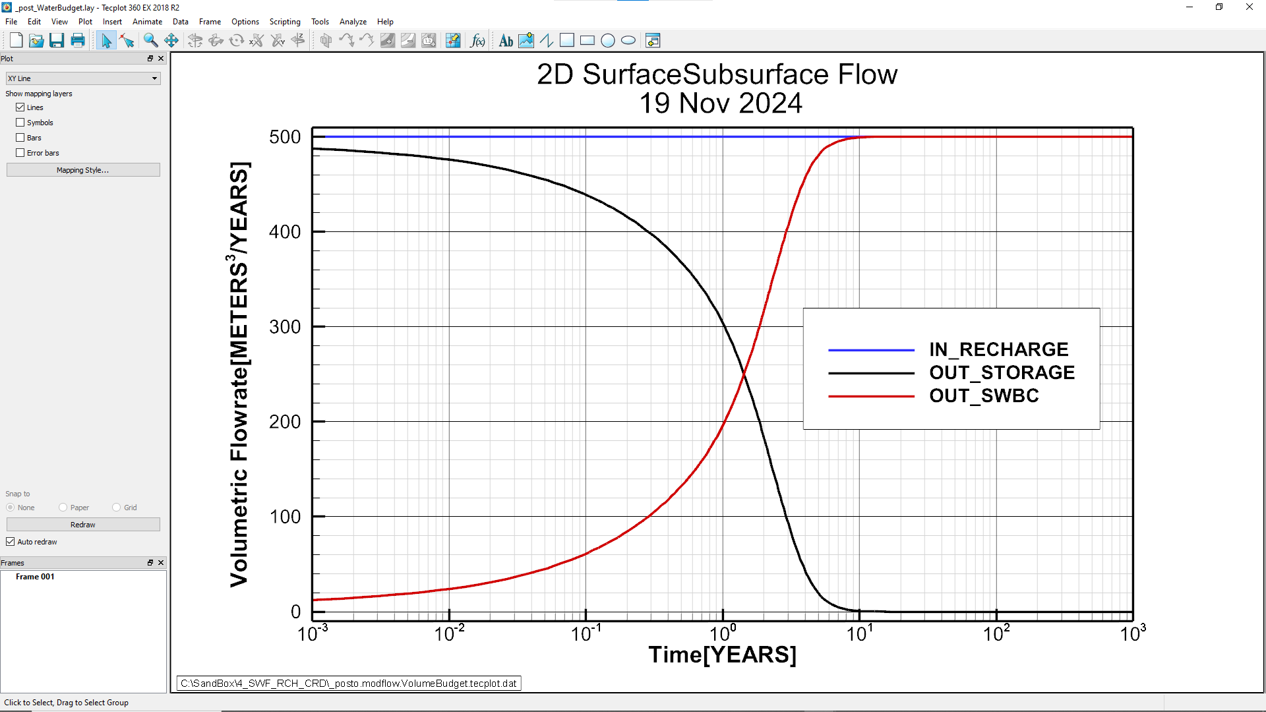
\includegraphics[width=\textwidth]{4_2_Budget}

This \tecplot\ frame has the following features and contents:
\begin{itemize}
  \item It is an {\sf XY Line} plot showing the volumetric flowrate versus time for selected components of the model.
  \item The name of the data file loaded into the frame is shown at the bottom left corner.
  \item The plot title, current date (on the day the file was loaded) and data set title ({\sf 4\_SWF\_RCH\_CRD}) are shown centred above the plot.
  \item The line legend is shown on the right side of the plot.
  \item The X-axis uses a log time scale.
\end{itemize}

The \tecplot\ date set information dialogue shows all of the variables available for plotting:

        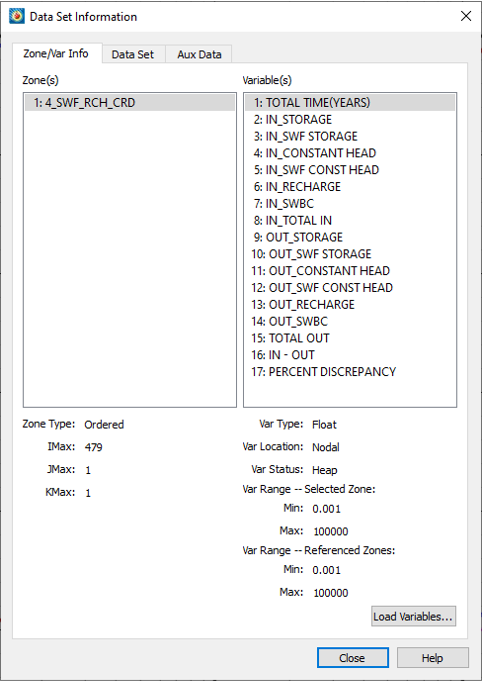
\includegraphics[width=.6\textwidth]{4_3_DataSetInfo}

Variable names are derived from the {\tt modflow.lst} file:
\begin{verbatim}
      VOLUMETRIC BUDGET FOR ENTIRE MODEL AT END OF TIME STEP  479 IN STRESS PERIOD    1
      ----------------------------------------------------------------------------- ---

         CUMULATIVE VOLUMES      L**3       RATES FOR THIS TIME STEP      L**3/T
         ------------------                 ------------------------

               IN:                                      IN:
               ---                                      ---
                 STORAGE =       3.0881E-04               STORAGE =       5.6023E-09
             SWF STORAGE =       9.9743E-03           SWF STORAGE =       2.1841E-13
           CONSTANT HEAD =           0.0000         CONSTANT HEAD =           0.0000
          SWF CONST HEAD =           0.0000        SWF CONST HEAD =           0.0000
                RECHARGE =    50000000.0000              RECHARGE =         500.0000
                    SWBC =           0.0000                  SWBC =           0.0000

                TOTAL IN =    50000000.0103              TOTAL IN =         500.0000

        ... etc

     PERCENT DISCREPANCY =           0.01     PERCENT DISCREPANCY =           0.01
\end{verbatim}


This example has a uniform recharge rate of 0.5 $meters/year$ which results in a total recharge of 500 $meters^{3}/year$ when multiplied by the 1000 $meter$ length of the cross-section. Initially, water comes out of storage then but this declines to zero at equilibrium.  Water exiting the surface water outflow critical depth boundary  {\sf OUT\_SWBC} is initially zero then rises to equal the toal recharge at equilibrium.  Fluid balance error {\sf IN-OUT} is essentially zero throughout the simulation.

The probe tool can be used in {\sf XY Line} plots to get exact variable values at a chosen location along the X or Y axis.  The cursor is shown as a vertical line if probing values on the X-axis (i.e.\ over time):

        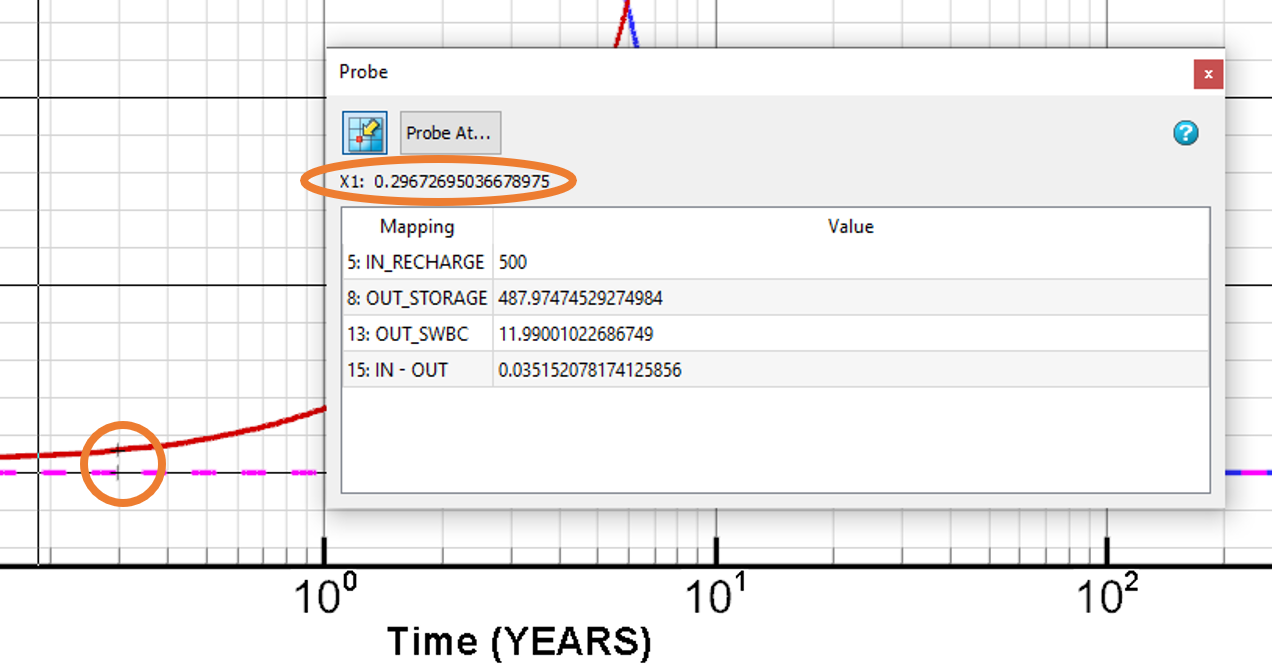
\includegraphics[width=\textwidth]{4_4_Probe}

Here, the location of the probe is shown by small vertical lines placed where the probe crossed the plotted lines.  The exact coordinate is given as {\sf X1: 0.2967...}  years.  At this early time, the {\sf OUT\_STORAGE} value is still near its initial value of 500 and the {\sf OUT\_SWBC} has just started rising.

A \tecplot\ layout file, \texttt{\_post.lay}, has been created for each verification example and  provides a quick way to view \mfus\ model solution results.  This result is from the example {\tt 6\_Abdul\_Prism\_Cell}:

        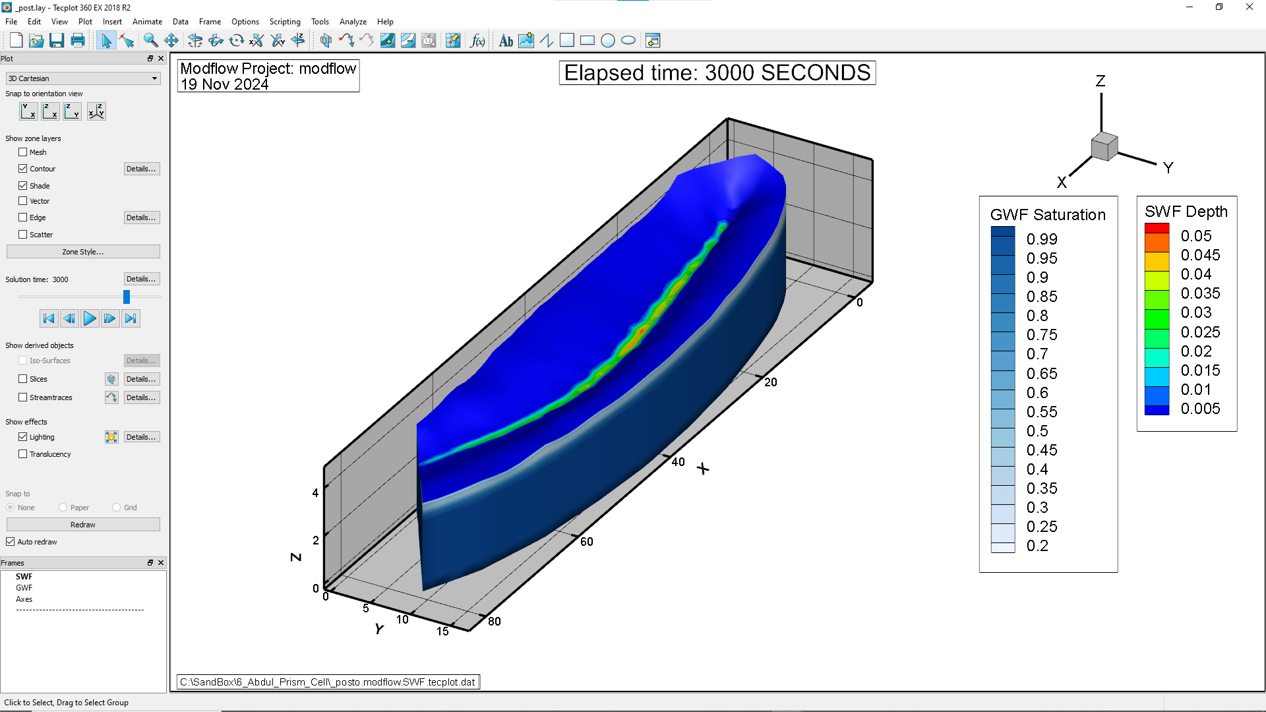
\includegraphics[width=\textwidth]{4_5_Post_Abdul}

The {\tt \_post.lay} layout file is similar to the {\tt \_build.lay} file shown earlier for the same problem: {\sf  SWF, GWF} and {\sf Axes} frames are visible (i.e. placed above the {\sf background} frame in the list).  The {\sf SWF} is currently active (i.e. the name is bolded) and placed at the front of the image (i.e. at the top of the list). It uses a different colormap to make it easier to distinguish the \gwf\ domain below.

In this case though, the contoured variables are {\sf SWF Depth} and {\sf GWF Saturation} results from the \mfus\ simulation.  The model output includes data for several output times, and the image above is showing conditions at a solution time of 3000 seconds, as indicated by the label near the top center of the plot.  The solution time shown is controlled by the slider and button controls near the centre of the {\sf Plot} frame on the left hand side of the image:

        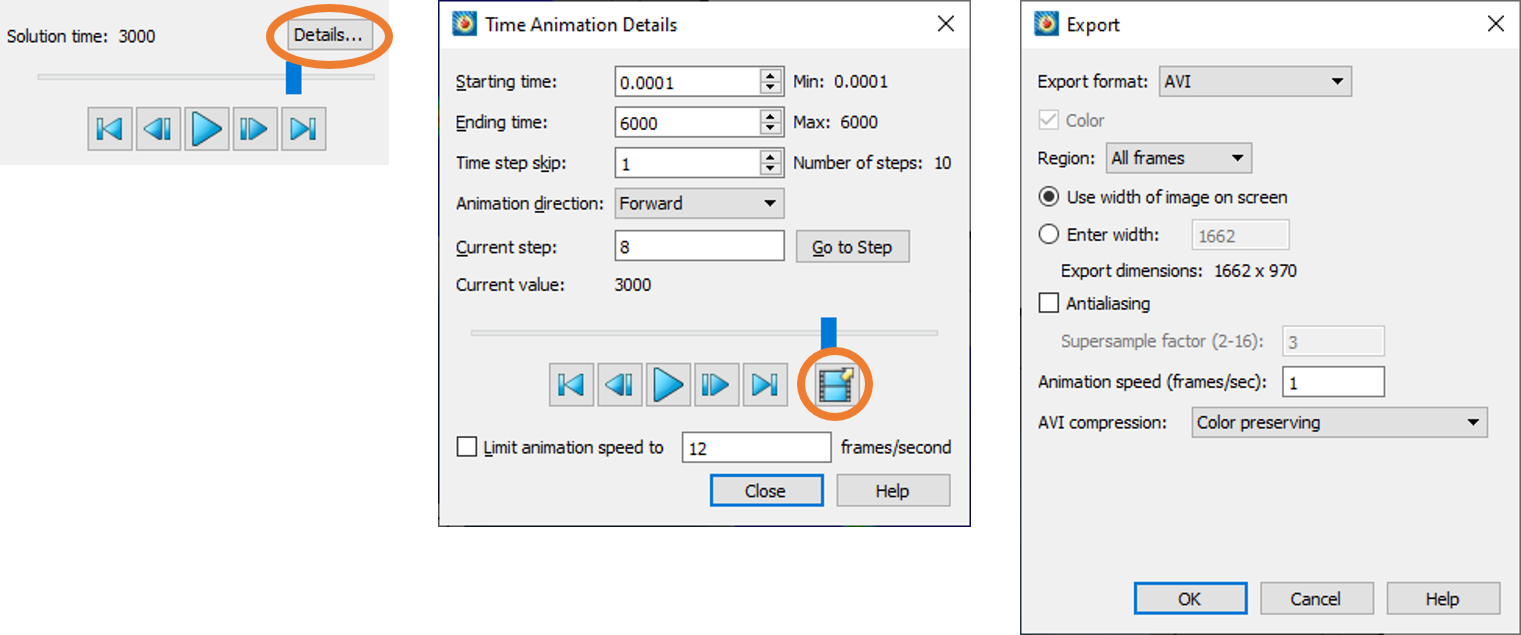
\includegraphics[width=.8\textwidth]{4_6_SolutionSlider}

The {\sf Details...} button leads to the {\sf Time animation details} dialogue which allows you to control and save animations of transient model results using the {\sf Export To File} button 
\includegraphics{ExportToFile}.  There is an example animation in  \texttt{$\backslash$MUT\_Examples-main$\backslash$\-6\_Abdul\_Prism\_Cell} folder in the powerpoint file {\tt Abdul Problem Animation.pptx}.  It used the settings shown in the {\sf Export} dialogue above to limit animations speed and write to an {\tt AVI}-formatted file.  This was then inserted in powerpoint where it can be viewed.

The {\sf Data Set Information} dialogues for the {\sf SWF} and {\sf GWF} frames are shown below:

        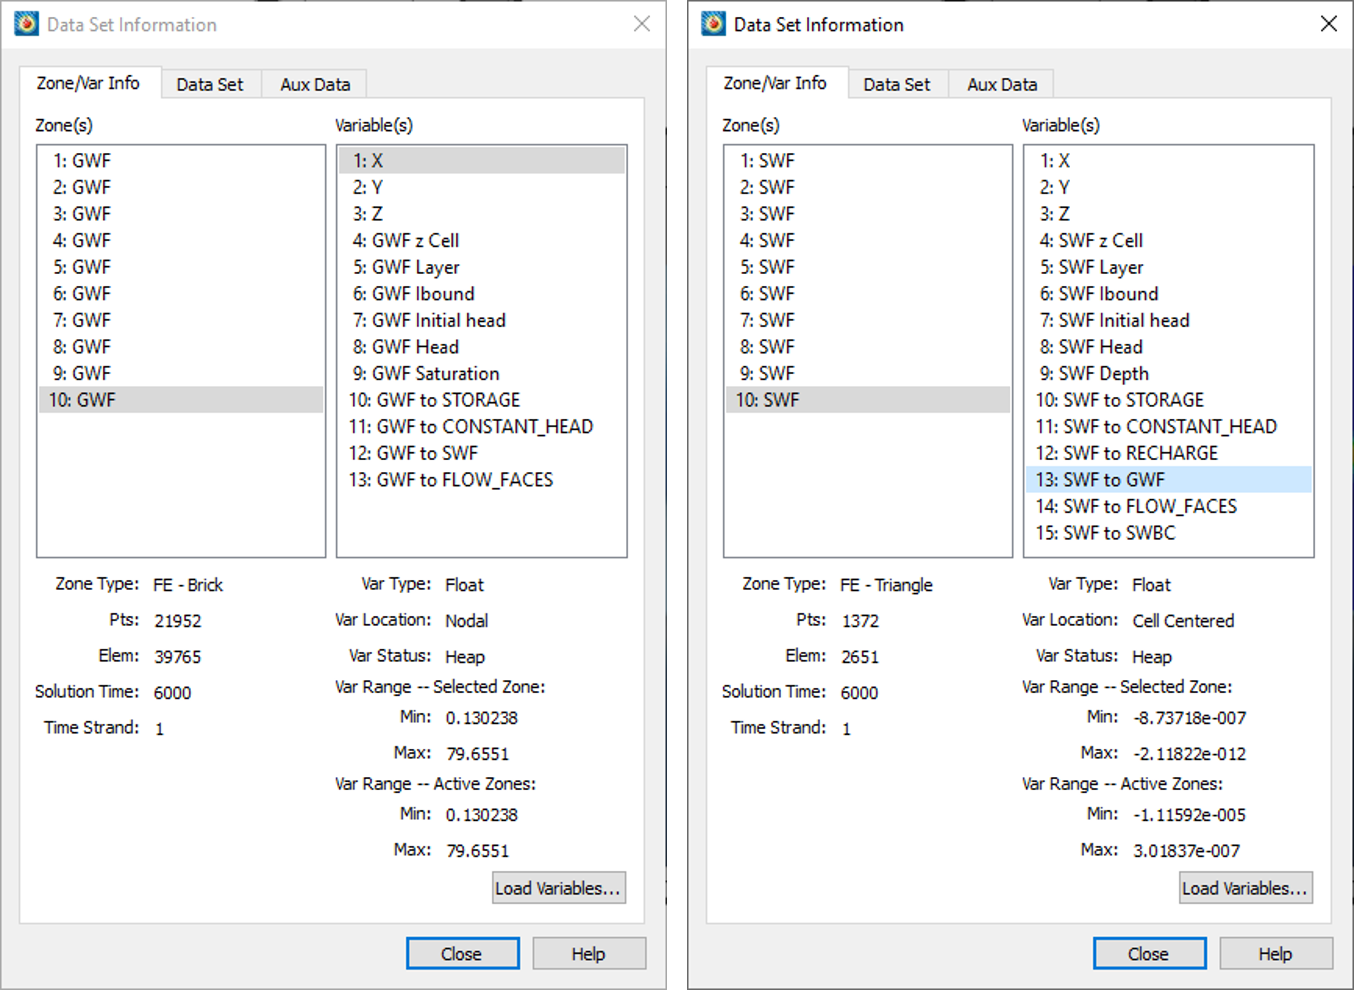
\includegraphics[width=.8\textwidth]{4_7_DatSetInfo}

These are similar to those shown earlier during the model build except there are now multiple {\sf Zone(s)}, one for each output time.  The {\sf Solution Time} (6000) is shown for the highlighted zone, in this case zone 10.

Included are these cell properties:
\begin{itemize}
    \item Elevation {\sf SWF z Cell} and {\sf GWF z Cell}.
    \item \mf\ layer number  {\sf SWF layer}and {\sf GWF layer}.
    \item \mf\ boundary number {\sf SWF Ibound} and {\sf GWF Ibound}.
    \item Initial head.
    \item Hydraulic head result.
    \item \gwf\ saturation and \swf\ depth.  These are stored in the \mf\ DDN (drawdown) file.
    \item In this case, cell-by-cell flows are stored in \gwf\ variables 10 to 13 and \swf\ variables 10 to 15.
\end{itemize}

The verification example {\tt 6\_Abdul\_MODHMS} layout file {\sf \_plot.lay} uses \tecplot\ value-blanking and the {\sf SWF Ibound} and {\sf GWF Ibound} to remove inactive cells, which have an IBOUND value of 0, from the plot:

        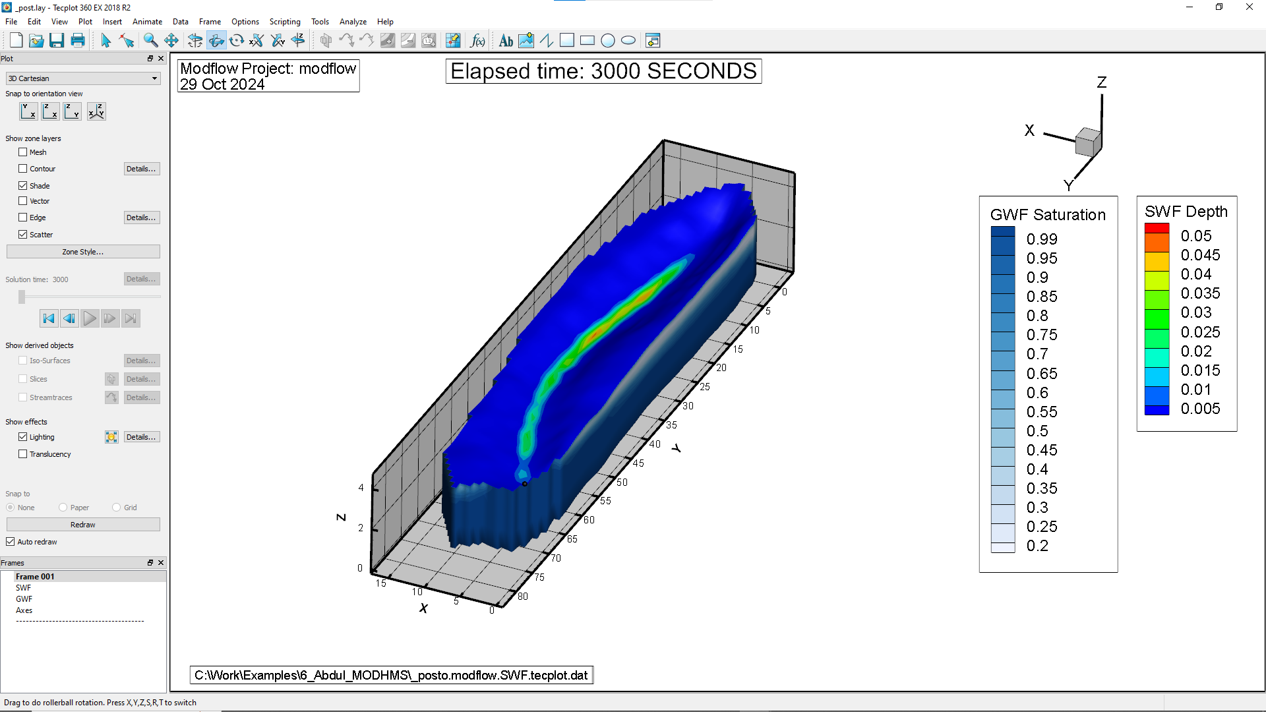
\includegraphics[width=.8\textwidth]{4_7a_MODHMS}


        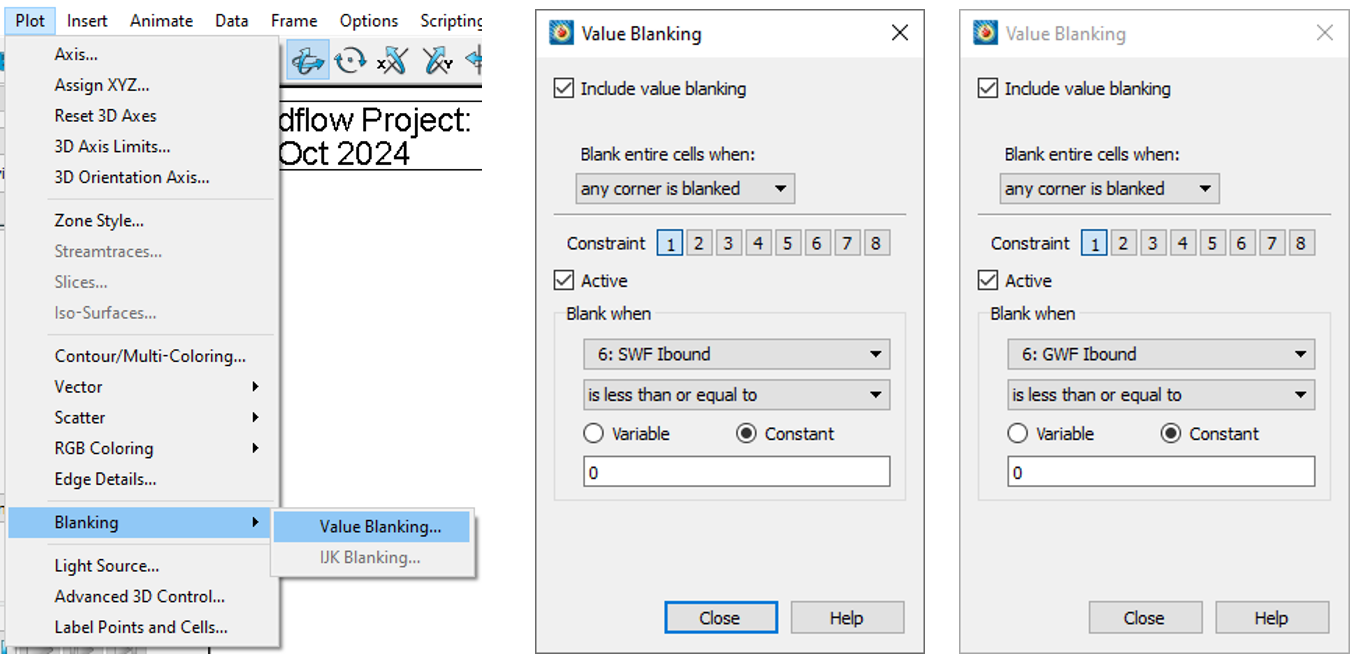
\includegraphics[width=.8\textwidth]{4_7b_ValueBlanking}

\index{\tecplot\ ! value blanking} 


        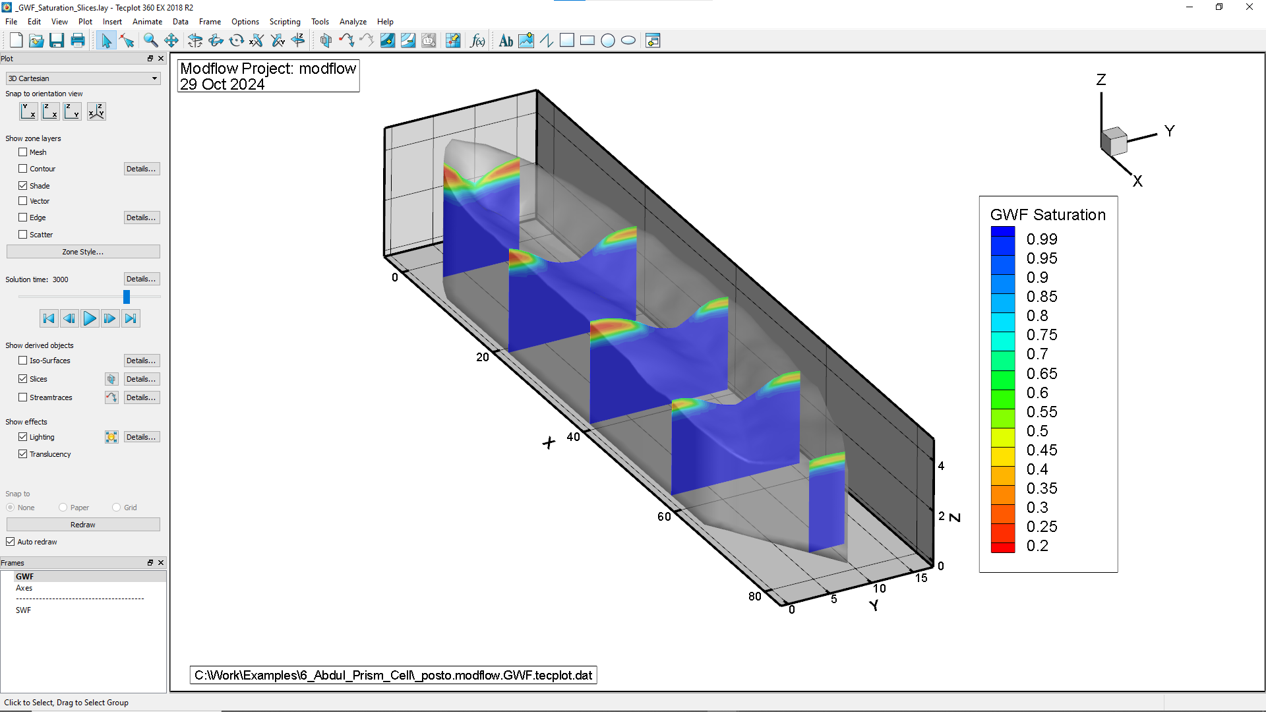
\includegraphics[width=.8\textwidth]{4_8_Slices}

\index{\tecplot\ ! slices and Fence diagrams}



\chapter{Examples}\label{texfile:Examples} 
    \section{Verification}
        \subsection{Unsaturated flow in a 1D Column} \input{1D_Build}
        \subsection{Unsaturated flow in a 2D Hillslope: Drains vs Surfacewater Flow}
        \subsection{Abdul's Experiment: 3D Unsaturated GroundwaterFlow }
    \section{Illustration}

\chapter{Tutorial}\label{chapter:Tutorial}




\printindex
\newpage

%\appendix
%\input{CookingNotes}
%\input{Scans}



\end{document}

% -----------------------------------------------------------------------------
